
\section{Ten years of FAIMS Mobile}

\begin{sectionframe} % Custom environment required for section slides
	\frametitle{Ten years of FAIMS Mobile}
	%\framesubtitle{Subtitle}

\begin{itemize}
    \item Research-specific,
    \item Generalised and customisable,
    \item Data collection focused, and
    \item Open-source software.
\end{itemize}


% 	This is on another line
\end{sectionframe}


%----------------------------------------------------------------------------------------

\begin{frame}{Research Specific}
 \begin{figure}[H]
    \centering
    \vspace{-0.5cm}
        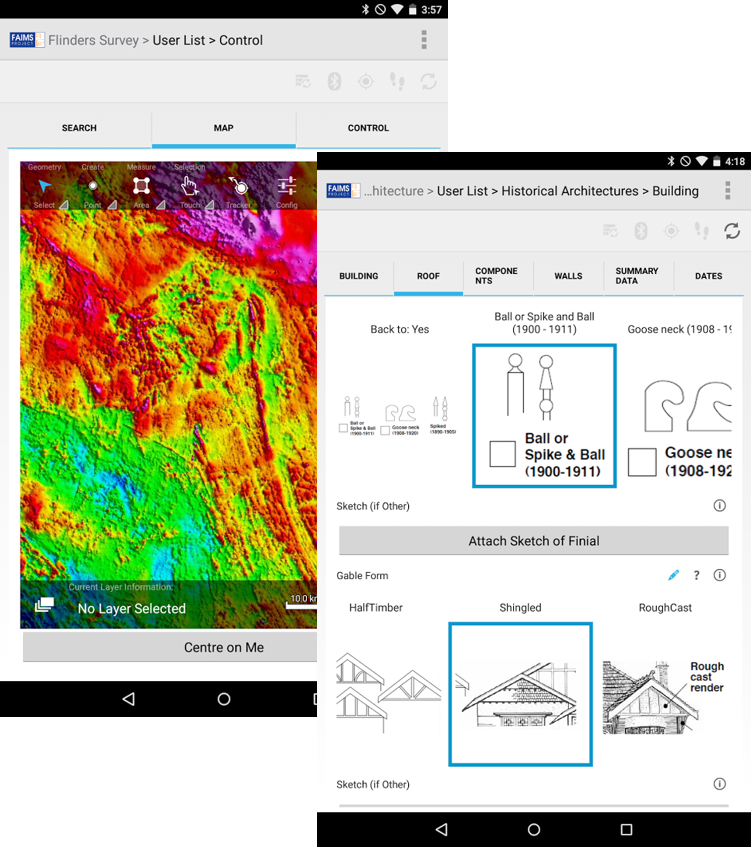
\includegraphics[height=.75\textheight]{figures/FAIMS-screenshots.png}
        \caption{FAIMS Mobile: GIS and `picture dictionaries'}
        \label{fig:FAIMS-mobile-screenshots}
 \end{figure}
\end{frame}

% %----------------------------------------------------------------------------------------

\begin{frame}{Key research-specific features}
	\begin{columns}[T]
		\begin{column}{0.45\textwidth}
        \begin{itemize}
            \item Customisable workflows.
            \item Offline capable.
            \item Complete data provenance / version history.
            \item Binds text, structured, geospatial, multimedia data.
            \item Mobile GIS with layers, raster and vector display, shape creation.
            \item Uses device and external sensors. 
            \item Multimedia file and metadata management.
        \end{itemize}
    \end{column}
	\begin{column}{0.45\textwidth}
        \begin{itemize}
            \item Validation and automation on device or server.
            \item Multilingual user-interface.
            \item Granular metadata: Notes and certainty for each field.
            \item Contextual help with images.
            \item Structured data can implement vocabularies / ontologies, LOD approaches.
            \item Data can be exported in a variety of formats, including custom exports.
        \end{itemize}
    \end{column}
\end{columns}
\end{frame}
%----------------------------------------------------------------------------------------

\begin{frame}{Generalised}
 \begin{figure}[H]
    \centering
        \vspace{-0.5cm}

        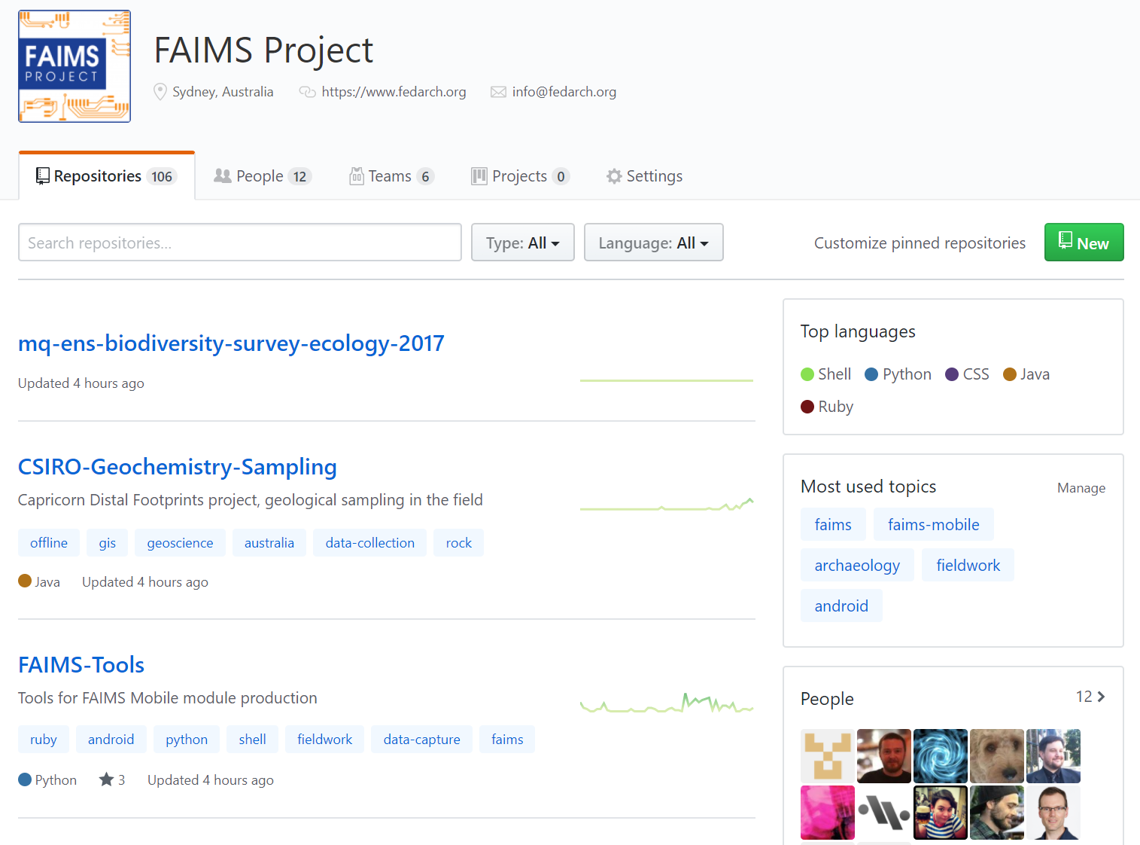
\includegraphics[height=.75\textheight]{figures/FAIMS-generalised.png}
        \caption{FAIMS Mobile customisations on GitHub}
        \label{fig:FAIMS-github}
 \end{figure}
\end{frame}
%----------------------------------------------------------------------------------------

\begin{frame}{Data-capture focused with flexible export}
 \begin{figure}[H]
    \centering
            \vspace{-0.5cm}

        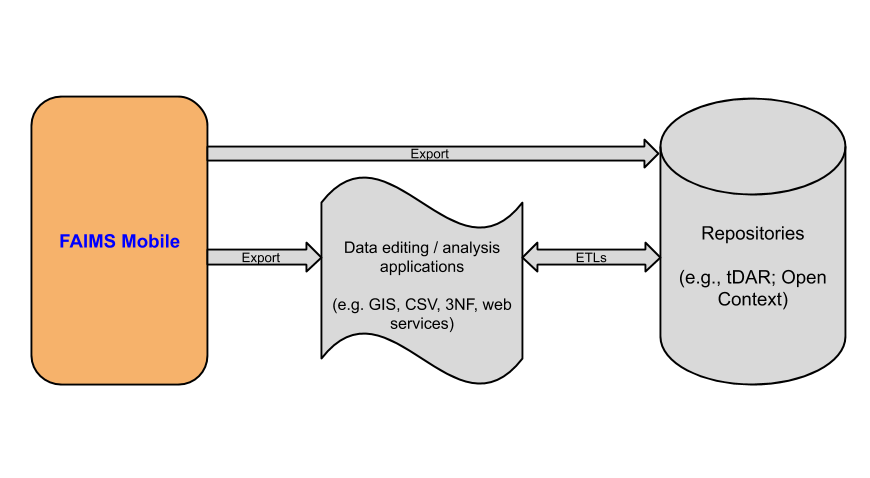
\includegraphics[height=.75\textheight]{figures/FAIMS-federation}
        \caption{FAIMS Mobile export workflows}
        \label{fig:FAIMS-federation}
 \end{figure}
\end{frame}
%----------------------------------------------------------------------------------------

\begin{frame}{Open Source}
 \begin{figure}[H]
    \centering
        
\includegraphics[width=.65\textwidth]{figures/asf_logo_url.png}
        
        \label{fig:FAIMS-github-OSS}
 \end{figure}
 
FAIMS Mobile v0.1-2.6 `core' code is licensed GPLv3; FAIMS 3.0 is licensed Apache 2.0; definition files are openly licensed (CC-BY); everything is on GitHub 

\end{frame}

%----------------------------------------------------------------------------------------

\begin{frame}{FAIMS 2.6 by the numbers}
 \begin{itemize}
        \item \textbf{64 field data capture workflows customised}.
        \item \textbf{48 workflows confirmed deployed} to field at over \textbf{40 projects}.
        \item \textbf{100s of users} logged \textbf{10,000s hours} on the platform.
        \item Deployments took place in disciplines including \textbf{archaeology, geoscience, ecology, oral history, ecology, }and \textbf{linguistics}.
    \end{itemize}
\end{frame}
%----------------------------------------------------------------------------------------


\begin{frame}{Example deployments}
 \begin{itemize}
        \item Indigenous Foodways in the Cape York Peninsula (UNE, archaeology)
        \item Khirbet el-Rai Excavations, Israel (Macquarie, archaeology).
        \item Landscape Archaeology at Lake Mungo (LTU, archaeology)
        \item Excavation at the Boncuklu Höyük, Turkey (UQ, archaeology).
        \item Tao River Archaeological Project, China (Harvard, archaeology).
        \item Proyecto Arqueològico Zaña Colonial, Peru (Brown, archaeology).
        \item The Malawi Earlier-Middle Stone Age Project (Yale, archaeology).
        \item Avian Ecology in NSW (Macquarie, ecology)
        \item The Greek-Australian Historical Archive (UNSW, oral history).
        \item Key Pluridisciplinary Advances on African Multilingualism, Cameroon (SUNY Buffalo, linguistics).
        \item Capricorn Distal Footprints Project (CSIRO, geological sampling).

    \end{itemize}
\end{frame}